\chapter{Market Survey}
The following products are available which provide similar fuctionality to our system

\section{Workscape}

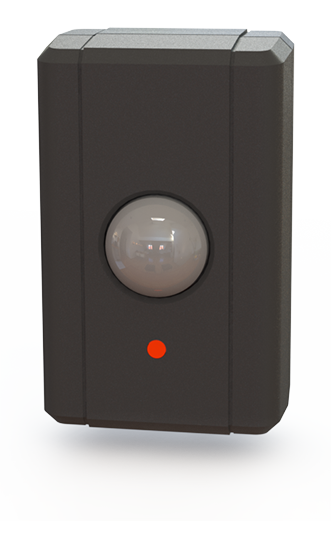
\includegraphics[scale=0.25]{Workscape1.png}
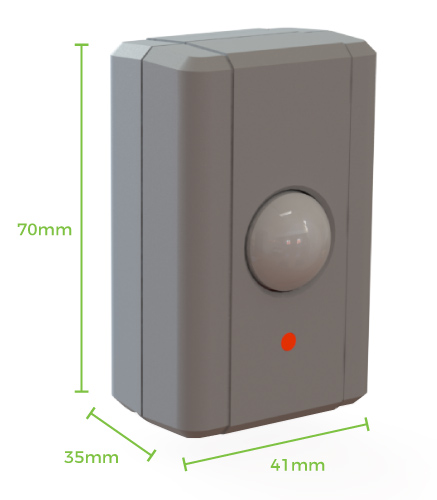
\includegraphics[scale=.5]{Workscape2.png}

\section{OccupEye}

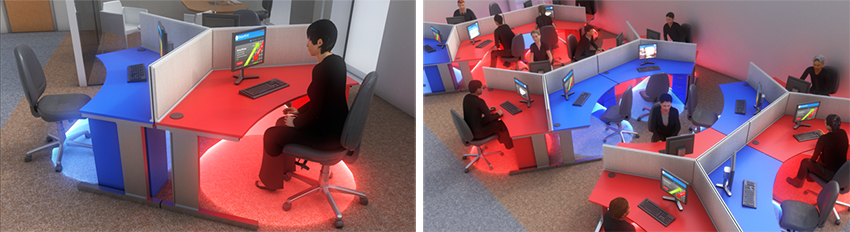
\includegraphics[scale=0.25]{HotColdDeskOccupEye.png}

\section{Workscape}
As sequentially operating digital computers implement the control algorithm, it is crucial to provide appropriate computing power. The required computing speed depends on the time constants involved. power electronics systems operate in `real time' which is a synonym of `natural time'. Therefore, the control system must synchronize its operations to real time. The correctness of a real-time system depends not only on the logical result of the computation but also on the time at which the results are produced. Real-time systems have to respond to externally generated stimuli within a finite and specified delay. Whereas a deadline can be missed occasionally in `soft real-time systems' such as on-line data banks, it is absolutely imperative for `hard real-time systems' that responses occur within the specified deadline on each and every occasion ~\cite{qing}. This does definitely apply to power electronic control systems. Digital control systems constitute discrete-time sampled systems. With regard to power electronic systems, real-time operation typically involves control and sampling cycles in the range of 20 - 200 $\mu s$ for normal operation. However, in case of fault situations, a reaction time of less than 1 $\mu s$ might be required ~\cite{mcc}.
 \section{Classification of Real-Time Simulation}
Testing and simulation of control algorithms is an
important phase in the development of embedded control
systems (ECS). Different types of simulation are possible  
during the design process of a controller~\cite{ram}~\cite{rain}, ranging
from simulation without time limitations, to partial real-time
simulation in which only some parts of the complete
control loop are simulated.
\par The initial functional evaluation of a control design is usually performed by off-line simulation of the control algorithm and the system. A successful evaluation leads to further tests and optimization under real-time conditions. These tests aim to improve the ability of a control design (1) to operate in real-time and (2) to interact with real equipment. Interaction with real equipment requires a large variety of interfaces. Currently the interaction with equipment relies increasingly on complex and powerful digital interfaces replacing analog interfaces to sensors and actuators. Digital interfaces generally yield a more noise immune data transfer and facilitate additional auxiliary features such as diagnostics.\par
A functional control prototype is required for the validation under real-time conditions. Usually the final control hardware is not yet available at this stage. Instead, rapid prototyping methods are used to provide an early functional real-time prototype of the control system. For this prototype, the functional behavior of the control system is reproduced by an emulator. The emulator requires flexible and powerful hardware structures in order to achieve real-time operation and interaction with either a real or a simulated environment.\par  
Real-time simulation allows comprehensive and safe tests in the laboratory if tests in the real environment are not feasible or desirable. It simulates the entire load system under normal and fault conditions. Digital simulation offers several appealing advantages over analog simulation with regard to the dynamic range of variables, flexibility and reproducibility of results for each performance etc. Digital real-time simulation is much more challenging than control system emulation because it has to operate five or ten times faster than control systems to avoid delays which may generate artificial low frequency effects. Thus, digital real-time simulation demands very high performance of its underlying hardware structure. The use of parallelism inherent in large systems is inevitable and has to be reflected in a similar parallelism in the simulator hardware.\par
  
